%\documentclass[10pt,twocolumn,letterpaper,draft]{article}
\documentclass[10pt,letterpaper]{ctexart}

\usepackage{cvpr}
\usepackage{graphicx}
\usepackage{wrapfig}
\usepackage{amsmath}
\newtheorem{myDef}{Definition}
\newtheorem{myTheo}{Theorem}

\usepackage{amssymb}
\usepackage{booktabs}
\usepackage{subfigure}
\usepackage{algorithm}
\usepackage{algorithmicx}
\usepackage{algpseudocode}
\usepackage{pythonhighlight}
\usepackage{xcolor}
\usepackage{listings}

\lstset{language=C++,
    basicstyle=\ttfamily,
    frame=single,
    keywordstyle=\color{blue}\ttfamily,
    stringstyle=\color{magenta}\ttfamily,
    commentstyle=\color{green}\ttfamily,
    morecomment=[l][\color{magenta}]{\#},
    morekeywords={*,uint_fast64_t}
}

\renewcommand{\labelenumi}{\alph{enumi}.} % Make numbering in the enumerate environment by letter rather than number (e.g. section 6)
\floatname{algorithm}{算法}
\renewcommand{\algorithmicrequire}{\textbf{输入:}}
\renewcommand{\algorithmicensure}{\textbf{输出:}}
\renewcommand{\lstlistingname}{代码清单}

\usepackage{enumitem}
\setenumerate[1]{itemsep=0pt,partopsep=0pt,parsep=\parskip,topsep=5pt}
\setitemize[1]{itemsep=0pt,partopsep=0pt,parsep=\parskip,topsep=5pt}
\setdescription{itemsep=0pt,partopsep=0pt,parsep=\parskip,topsep=5pt}

% Include other packages here, before hyperref.

% If you comment hyperref and then uncomment it, you should delete
% egpaper.aux before re-running latex.  (Or just hit 'q' on the first latex
% run, let it finish, and you should be clear).
\usepackage[pagebackref=true,breaklinks=true,letterpaper=true,colorlinks,bookmarks=false]{hyperref}


\cvprfinalcopy % *** Uncomment this line for the final submission

\def\cvprPaperID{159} % *** Enter the CVPR Paper ID here
\def\httilde{\mbox{\tt\raisebox{-.5ex}{\symbol{126}}}}

\newcommand{\mypara}[1]{\paragraph{#1.}}

\graphicspath{{figures/}}

% Pages are numbered in submission mode, and unnumbered in camera-ready
%\ifcvprfinal\pagestyle{empty}\fi
\setcounter{page}{1}


%\begin{CJK*}{GBK}{song}

\newcommand{\figref}[1]{图\ref{#1}}
\newcommand{\tabref}[1]{表\ref{#1}}
\newcommand{\equref}[1]{式\ref{#1}}
\newcommand{\secref}[1]{第\ref{#1}节}

\ctexset{
  section={
    % name={,、},
    number={\chinese{section}},
    format={\heiti},
    beforeskip={0.1ex},
    afterskip={0.1ex},
    % aftername={\nobreak},
    indent={\parindent},
    },
}
\usepackage{zhnumber}

\newcommand\zhsubsec[1]{{% 中文小节
\bfseries{
\stepcounter{subsection}(\zhnum{subsection}){#1}}
\vspace{0.1pt}%
}}

%%%%%%%%% TITLE

\begin{document}
\pagestyle{plain}
\title{
    \begin{center}
        \phantom{Start!}
    	  \vspace{2cm}
        \center{\zihao{1} 中山大学数据科学与计算机学院}
        \center{\zihao{2} 计算机科学与技术专业-人工智能}
        \center{\zihao{2} 本科生实验报告}
        \center{(2018-2019学年秋季学期)}
    \end{center}
}
\maketitle

\begin{center}
    \setlength{\baselineskip}{40pt}
    \vspace{1cm}
    \zihao{-2}
    \center{
        \begin{tabular}{cc}
      	学\qquad 号:& \underline{~~~~~~16337113~~~~~~}  \\
      	姓\qquad 名:& \underline{~~~~~~~劳马东~~~~~~~}  \\
        教学班级:   & \underline{~~~~~教务2班~~~~~}  \\
      	专\qquad 业:& \underline{~~~~~~~~~超算~~~~~~~~}  \\
      	\end{tabular}
    }
\end{center}
\pagebreak

%%%%%%%%% BODY TEXT %%%%%%%%%%%%%%%%%%%%%%%%%%%%%%%%%%%%%%%%
\section{实验题目}
实现变量消元算法的$inference, multiply, sumout$和$restrict$函数,求解:
\par P(Alarm)
\par P(J \&\& $\sim$M)
\par P(A | J \&\& $\sim$M)
\par P(B | A)
\par P(B | J \&\& $\sim$M)
\par P(J \&\& $\sim$M | $\sim$B)

\section{实验内容}
  \zhsubsec{因子(factors)}
  \par 在变量消元过程中,经常会遇到像这样的式子——$\sum_APr(A)\sum_BPr(B)Pr(C|A,B)$,它实际上是求$Pr(A, B, C)$。
  我们将先验分布$Pr(A)$、$Pr(B)$和条件分布$Pr(C|A,B)$抽象为因子,统一表示为$f(A)$、$f(B)$和$f(C,A,B)$。因子$f(V_1, V_2, ...,V_n)$
  是随机变量集合$\{V_1, V_2, ...,V_n\}$到非负实数域的映射,每个随机变量实例化后的$f(v_1, v_2, ..., v_n)$是对应的条件概率或联合概率。
  例如,$f(a)=Pr(A=a)$,$f(a,b,c)=Pr(c|a,b)$。
  \par 个人认为,引入因子的原因,一方面是便于书写,不必考虑随机变量之间的关系(如哪些变量是前提);另一方面是更好地重用因子,因为在推理过程中
  有很多重复计算,如果保存推理过程中得到的因子,结合因子涉及的随机变量,能很快发现哪些因子可以重用,减少不必要计算。

  \zhsubsec{因子的基本操作}
  \begin{enumerate}[itemindent=2em,label=\arabic*、]
    \item 对某个变量V求和(sum-out)
    \par \qquad 假设存在因子$f(V_1, V_2, ..., V_n)$,它要在随机变量$V_1$上求和,从而产生一个新的因子,过程如下:
    \begin{enumerate}[itemindent=2em,label=(\arabic*)]
      \item $\forall v \in V_1$,将除$V_1$外其余变量取值相同的$f(v, V_2, ..., V_n)$相加;
      \item 将$V_1$从$f$中删除,得到一个新的因子$g(V_2, ..., V_n)$,其中$g(v_2, ..., v_n)=\sum_{v \in V_1}f(v, v_2, ..., v_n)$。
    \end{enumerate}

    \begin{algorithm}
      \caption{因子求和}
      \begin{algorithmic}[1] %每行显示行号
          \Function {$sumout$}{$f, i$}
          \Require 因子$f$,$f$要消除的变量的下标$i$
          \Ensure 求和后的新因子$g$
            \State $V_1, V_2, ..., V_n \gets f.variables$
            \State $g \gets$ new factor with variables $\{V_1, ..., V_{i-1}, V_{i+1}, ..., V_n\}$
            \For{\textbf{each} tuple $(v_1, ..., v_{i-1}, v_{i+1}, ..., v_n)\ \in\ g$}
              \State $g[(v_1, ..., v_{i-1}, v_{i+1}, ..., v_n)] \gets 0$
            \EndFor

            \For{\textbf{each} tuple $(v_1, v_2, ..., v_n)\ \in\ f$}
              \State $g[(v_1, ..., v_{i-1}, v_{i+1}, ..., v_n)] \gets g[(v_1, ..., v_{i-1}, v_{i+1}, ..., v_n)] + f[(v_1, v_2, ..., v_n)]$
            \EndFor
            \State \Return $g$
          \EndFunction
      \end{algorithmic}
    \end{algorithm}

    \item 因子相乘(factor multiplication)
    \par \qquad 假设因子$f(A,B)$与$g(B, C)$具有相同的变量$B$,则$f$与$g$的乘积,记为$h(A,B,C)=f(A,B) \times g(B,C)$,是它们的自然连接,概率是对应元组概率的乘积。
    例如,对于\tabref{tab:mul}中的例子,给出$f(A,B)$和$g(B,C)$各种取值的概率,$ab$与$bc$自然连接产生$abc$,它的概率是$f(a,b) \times g(b,c)=0.9\times 0.7=0.63$,
    $ab$与$\sim bc$自然连接时由于$b \neq \sim b$,不产生结果。同理可以得出其余自然连接的结果。
    \begin{table}[!htbp]
      \centering
      \begin{tabular}{|c|c|c|c|c|c|c|c|}
          \hline
          \multicolumn{2}{|c|}{f(A, B)} & \multicolumn{2}{|c|}{g(B, C)} & \multicolumn{4}{|c|}{h(A, B, C)} \\
          \hline
          ab & 0.9 & bc & 0.7 & abc & 0.63 & ab$\sim$c & 0.27\\
          a$\sim$b & 0.1 & b$\sim$c & 0.3 & a$\sim$bc & 0.08 & a$\sim$b$\sim$c & 0.02\\
          $\sim$ab & 0.4 & $\sim$bc & 0.8 & $\sim$abc & 0.28 & $\sim$ab$\sim$c & 0.12\\
          $\sim$a$\sim$b & 0.6 & $\sim$b$\sim$c & 0.2 & $\sim$a$\sim$bc & 0.48 & $\sim$a$\sim$b$\sim$c & 0.27\\
          \hline
      \end{tabular}
      \caption{因子相乘示例}\label{tab:mul}
    \end{table}

    \begin{algorithm}
      \caption{因子相乘}
      \begin{algorithmic}[1] %每行显示行号
          \Function {$multiply$}{$f, g$}
          \Require 因子$f$和$g$
          \Ensure 相乘得到的新因子$h$
            \State $common \gets f.variables \cap g.variables$
            \State $h \gets$ new factor with variables $f.variables \cup g.variables$
            \For{\textbf{each} tuple $(x_1,x_2, ..., x_m) \in f$}
              \For{\textbf{each} tuple $(y_1, y_2, ..., y_n) \in g$}
                \If{$(x_1,x_2, ..., x_m)$ is the same as $(y_1, y_2, ..., y_n)$ on $common$}
                  \State $h[(x_1,x_2, ..., x_m) \cup (y_1, y_2, ..., y_m)] \gets f[(x_1,x_2, ..., x_m)] \times g[(y_1, y_2, ..., y_n)]$
                \EndIf
              \EndFor
            \EndFor
            \State \Return $h$
          \EndFunction
      \end{algorithmic}
    \end{algorithm}

  \end{enumerate}

  \zhsubsec {变量消元过程}
  \par 假设给定一个贝叶斯网络,CPT表为$F$,查询变量为$Q$,证据变量$E$带观察值$e$,剩余未消除的变量集合为$Z$,计算$Pr(Q|E)$。
  \begin{enumerate}[itemindent=2em,label=\arabic*、]
    \item 证据变量赋值(Restriction)
    \par \qquad 对于$F$中的所有包含变量$E$的因子$f$,将它上$E \neq e$的元组删除,只保留那些$E == e$的元组,最后产生一个新的因子$g$。
    将$g$加入$F$,将$f$从$F$中删除。如果$f$只包含$E$这一个变量,$g$将是一个“常量”因子,可不放入$F$中。
    \item 按顺序消除变量
    \par \qquad 对于给定消元顺序中的每个变量$Z_j \in Z$,用以下步骤消除它:
    \begin{itemize}
      \item 假设因子$f_1,f_2,...,f_k$包含变量$Z_j$;
      \item 计算新因子$g_j = \sum_{Z_j}\prod_{i=1}^kf_i$;
      \item 将$f_1,f_2,...,f_k$从$F$中删除,并加入新的因子$g_j$。
    \end{itemize}
    \item 含查询变量的因子相乘
    \par \qquad 消除完成后,$Z$中剩下的因子都是只和$Q$相关的因子,记为$f_1(Q),f_2(Q),...,f_k(Q)$,$f(Q) = \prod_{i=1}^kf_i(Q)$。
    \item 归一化
    \par \qquad $f(Q)$上的概率相加的和不一定是1,尤其是在求条件概率时概率和通常大于1,因此需要归一化,即$\forall t \in f, f[t] = \alpha f[t]$,
    其中$\alpha = \frac{1}{\sum_{t \in f} f[t]}$。
  \end{enumerate}

  \par 现在考虑一个具体的例子,如\figref{fig:ve_example}。在图右边的贝叶斯网络中,变量$C$的父节点是$A$和$B$,变量$D$的父节点是$C$,因此CPT中的因子就是$f_1(A)$、
  $f_2(B)$、$f_3(A,B,C)$、$f_4(C,D)$。现在,在观察到证据变量$D=d$的前提下,计算查询变量$A$的概率,即$Pr(A|D=d)$,变量消元的顺序是$C$、$B$。
  \begin{figure}[H]
    \centering
    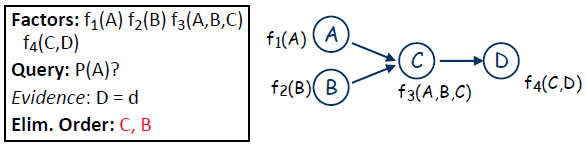
\includegraphics[width=0.6\textwidth]{ve_example.PNG}
    \caption{变量消元例子}\label{fig:ve_example}
  \end{figure}

  \par 第一步,证据变量赋值。证据变量是$D$,因子$f_4(C,D)$与$D$相关,于是限制$f_4$上$D$的值为$d$,产生新的因子$f_5(C)$;
  \par 第二步,按给定顺序消除变量。首先消除$C$,计算并添加因子$f_6(A,B) = \sum_Cf_5(C)f_3(A,B,C)$,删除因子$f_3$和$f_5$;
  然后消除$B$,计算并添加因子$f_7(A)=\sum_B f_2(B)f_6(A,B)$,删除$f_2$和$f_6$。
  \par 第三部,现在剩下的因子是$f_1(A)$和$f_7(A)$,它们都只和$A$相关,计算$f_1(A)\times f_7(A)$。
  \par 最后,归一化。$Pr(A|D=d)=\alpha f_1(A)\times f_7(A)$,其中$\alpha=\frac{1}{\sum_A f_1(A)\times f_7(A)}$。

\section{关键代码}
\begin{enumerate}[itemindent=2em,label=\arabic*、]
  \item 因子求和
  \par \qquad 首先是将要求和的变量$variable$从变量列表中删除,得到新的变量列表$new\_var\_list$,$var\_index$是$variable$在旧变量列表中的下标。
  \par \qquad 然后,遍历$cpt$中的每一个键值对,键是变量取值,值是对应的概率。新的键$new\_k$由旧键删除第$var\_index$个元素产生,新的值时相同$new\_k$对应概率的累加和。
  \begin{python}
def sum_out(self, variable):
  # 找到variable在var_list中的下标,并将其删除产生新的变量列表
  var_index, new_var_list = self.without(variable)
  new_cpt = dict()    # 利用字典统计概率的累加和
  for k, v in self.cpt.items():
    new_k = k[:var_index] + k[var_index + 1:]   # 用分片实现字符串删除第var_index个元素
    new_pro = new_cpt.get(new_k, 0) + v
    new_cpt[new_k] = new_pro
  # 尝试一个新的因子,变量列表是new_var_list,概率表是new_cpt
  new_node = Node('f' + str(new_var_list), new_var_list)
  new_node.set_cpt(new_cpt)
  return new_node
  \end{python}

  \newpage
  \item 因子相乘
  \par \qquad 如上文所述,因子相乘其实是自然连接的过程。因此,第一步是找到两个因子相同的变量集合,这借助于$interaction$函数,它返回两个列表
  共有的元素列表。然后,使用一个二重循环变量两个因子$cpt$表上的每一项,用$join$函数在$common$上连接两个项,返回$t1 \cup t2$,如果这两个项无法连接将返回$None$。
  \begin{python}
def multiply(self, factor):
  new_cpt = dict()
  common = []
  # 求两个因子的交集,并在common中添加这些交集变量对应的下标
  for c in Util.interaction(self.var_list, factor.var_list):
    common.append((self.get_var_index(c), factor.get_var_index(c)))
  for t1, v1 in self.cpt.items():
    for t2, v2 in factor.cpt.items():
      k = Util.join(t1, t2, common) # 按common上的属性,自然连接t1和t2
      if k is not None:
        new_cpt[k] = v1 * v2
  new_var_list = self.var_list + factor.var_list
  for i, _ in common:   # 求并集,删除self.var_list + factor.var_list中重复的元素
    new_var_list.pop(i)
  new_node = Node('f' + str(new_var_list), new_var_list)
  new_node.set_cpt(new_cpt)
  return new_node
  \end{python}

  \item 按顺序消除变量
  \par \qquad 在消除的过程中,将因子列表$factor\_list$看做一个队列,每次取队头元素,如果它包含要消除的变量$var$,就将它和同样具有$var$
  变量的因子相乘,否则重新将它放入队列。

  \begin{python}
for var in ordered_list_of_hidden_variables:
  new_f = None
  for i in range(len(factor_list)):
    factor = factor_list.pop(0)   # 移除队头的因子
    if var in factor.var_list:
      # 将所有含var变量的因子相乘
      if new_f is None:
        new_f = factor
      else:
        new_f = new_f.multiply(factor)
    else:   # 因子不包含var变量,不能相乘,重新放入队列
      factor_list.append(factor)
  if new_f is not None:   # 相乘后是求和操作
    new_f = new_f.sum_out(var)
    factor_list.append(new_f)
  \end{python}
  \item 归一化
  \begin{python}
def normalize(cpt, query_variables):
  n = len(query_variables)  # 默认因子的前n个是非条件
  totals = dict()
  for k, v in cpt.items():
    totals[k[n:]] = totals.get(k[n:], 0) + v
  for k in cpt:
    cpt[k] /= totals[k[n:]]
  \end{python}
\end{enumerate}

\section{实验结果}
\begin{table}[!htbp]
  \begin{tabular}{c|c|c|c|c|c}
    \toprule
      & 证据变量 & 查询变量 & 消元顺序 & key & 概率\\
    \hline
    P(A) & - & 'A' & 'B'、'E'、'J'、'M' & '1' & 0.002516442\\
    P(J \&\& $\sim$M) & - & 'J'、'M' & 'B'、'E'、'A' & '10' & 0.050054875461\\
    P(A | J \&\& $\sim$M) & 'J': '1', 'M': '0' & 'A' & 'B'、'E' & '1' & 0.013573889331307633\\
    P(B | A) & 'A': '1' & 'B' & 'E'、'J'、'M' & '1' & 0.373551228281836\\
    P(B | J \&\& $\sim$M) & 'J': '1', 'M': '0' & 'B' & 'E'、'A' & '1' & 0.0051298581334013015\\
    P(J \&\& $\sim$M | $\sim$B) & 'B': '0' & 'J'、'M' & 'E'、'A' & '10' & 0.049847949\\
    \bottomrule
  \end{tabular}
\end{table}
\end{document}

